\documentclass[runningheads]{llncs}
\usepackage{graphicx}
\usepackage{booktabs}
\usepackage{amsmath}

\begin{document}

\title{No Single Uncertainty-Quantification Method Reliably Flags Domain-Shift Failure in a Cervical Cytology Classifier}
\titlerunning{No Single UQ Method Reliably Flags Domain-Shift Failure}

\author{Anonymous Author(s)}
\authorrunning{Anonymous Author(s)}
\institute{Submitted for double-blind review}

\maketitle

\begin{abstract}
A vision transformer that classifies cervical cytology images with 96\%+
in-distribution accuracy but collapses to near- or below-chance accuracy
under real cross-institution domain shift -- as we previously showed
EfficientViT-M0 does on the Mendeley LBC dataset -- is only as dangerous as
its confidence is falsely high when it fails. We compare four
uncertainty-quantification methods on that exact backbone, using each
method's own cheapest native confidence signal (temperature-scaled
max-softmax, MC Dropout entropy, evidential vacuity, deep-ensemble
variance), evaluated in distribution and on both a moderate (Herlev) and
severe (Mendeley LBC) external shift. In distribution, three of the four
methods calibrate well (expected calibration error 0.012--0.013);
evidential deep learning's raw belief masses are markedly less calibrated
(0.159) at matched point accuracy. Under moderate shift, a five-member
deep ensemble is unambiguously the best method by every metric measured.
Under severe shift -- the condition that matters most, since it is where
the backbone is known to fail -- the ranking inverts in our original run:
MC Dropout's entropy is the only signal that substantially improves
shift-failure detection over the uncalibrated baseline (risk-coverage AUC
0.515 to 0.285), while the deep ensemble's advantage does not transfer
(0.473, barely better than baseline) despite being the clear winner on the
milder shift. A follow-up paired-bootstrap significance test, run on an
independently retrained MC Dropout model (identical seed, recipe, and
data), does not reproduce this advantage: the retrained model's Mendeley
LBC risk-coverage AUC is 0.503, not 0.285, and is statistically
indistinguishable from the deep ensemble's 0.474 (95\% CI for the
difference $[-0.066, 0.010]$, one-sided $p=0.929$) -- so the reported
severe-shift rank inversion, while real for the specific trained model in
Table~1, is not a stable property that survives retraining under an
identical recipe. No method reaches a reliable abstention operating point
on the severe shift condition in either run: even MC Dropout's best
selective accuracy at 90\% coverage (0.583, on a binary task, from the
original run) is barely better than chance after abstaining on the
least-confident decile. We conclude that uncertainty-method ranking is
itself shift-magnitude-dependent and, on this severe-shift condition, not
even stable across retraining of the same method -- so no single fixed
uncertainty-quantification choice, however it performed in one training
run, can be assumed safe across the range of shift severity a deployed
screening tool will encounter.

\keywords{Uncertainty quantification \and Calibration \and Domain shift \and Selective prediction \and Cervical cytology}
\end{abstract}

\section{Introduction}

A model that fails silently -- misclassifying confidently under
conditions its training data did not cover -- is more dangerous in a
screening context than one that fails and flags the failure. We previously
established that this is not a hypothetical concern for a lightweight
cervical cytology classifier: EfficientViT-M0, the best in-distribution
model across a 12-model registry, is simultaneously the worst-performing
model under cross-dataset domain shift, dropping below the chance floor on
the more severe of two external cytology datasets tested. This paper asks
the natural next question: does any standard uncertainty-quantification
method's own native confidence signal correctly detect that specific
failure, using only the cheapest version of each method (a single native
signal, not a method-specific post-hoc correction layered on top) so the
comparison reflects what a deployed system would actually have access to
without extra engineering?

Our contributions are fivefold. First, a four-method uncertainty-
quantification comparison (temperature-scaled softmax, MC Dropout,
evidential deep learning, deep ensembles) on a backbone with a documented,
severe, real (not synthetic) distribution-shift failure mode, rather than
a synthetic corruption benchmark. Second, evidence that uncertainty-method
ranking itself depends on shift severity: the method that wins under
moderate shift (deep ensemble) is not the method that wins under severe
shift (MC Dropout) in our original run, and the gap between them under
severe shift is large (0.473 vs.\ 0.285 risk-coverage AUC) while their gap
under moderate shift favors the ensemble even more strongly (0.147 vs.\
0.203). Third, a direct, quantified answer to whether any of the four
methods reaches a \emph{reliable} abstention policy under severe shift:
none does, and we report the closest result (MC Dropout, 0.583 selective
accuracy at 90\% coverage) as still practically insufficient for an
``abstain and refer'' deployment policy, rather than rounding it up to a
success. Fourth, a methods-level finding independent of the uncertainty
comparison itself: MC Dropout is completely degenerate on this exact
backbone unless a code-level fix is applied before training, not just at
inference (Section~3.3) -- a reproducibility hazard for anyone applying MC
Dropout to a similarly-configured timm model without checking. Fifth, a
significance test that complicates the second contribution rather than
simply confirming it: retraining MC Dropout once more under the identical
seed and recipe used for Table~1 does not reproduce its reported
severe-shift advantage (risk-coverage AUC 0.503 versus the original run's
0.285), and a paired bootstrap test on this retrained run finds no
statistically significant difference from the deep ensemble at all --
meaning the specific rank inversion reported here should be read as a
property of one trained model, not a stable property of the method,
which is itself a load-bearing caution for any paper (including this one)
that reports a single-training-run method comparison as if it were a
method-level fact.

\section{Related Work}

\subsection{Post-hoc calibration and its limits under shift}

Temperature scaling \cite{guo2017calibration} remains the standard
post-hoc softmax calibration baseline: a single scalar fit on a held-out
split rescales logits so that in-distribution confidence matches
empirical accuracy, at essentially zero added inference cost. It is a
strong in-distribution baseline (consistent with this paper's Table~1) but
is a purely in-distribution correction by construction -- it cannot
introduce information the model did not already encode about
out-of-distribution inputs, which is exactly why it is the weakest signal
here once shift severity increases (Table~1, right-hand columns). This
motivates comparing it against methods that inject additional
signal at training or inference time rather than only recalibrating a
fixed model's existing outputs.

\subsection{Multi-pass and ensemble uncertainty}

MC Dropout \cite{gal2016dropout} approximates Bayesian inference by
keeping dropout active at test time and treating the spread across
repeated stochastic forward passes as an uncertainty signal, at a cost
proportional to the number of passes. Deep ensembles
\cite{lakshminarayanan2017ensembles} instead train several independently-
initialized models and use their disagreement, at a cost proportional to
ensemble size; empirically, ensemble diversity has been argued in the
broader literature to capture a different, complementary source of
uncertainty (functional diversity across independently-trained models)
than a single model's own stochastic-forward-pass variance, which is
consistent with this paper's finding that the two methods are not
redundant with each other -- they win under different shift severities
rather than one strictly dominating the other.

\subsection{Single-pass uncertainty and evidential learning}

Evidential deep learning \cite{sensoy2018evidential} reframes
classification as Dirichlet evidence accumulation, producing a
single-pass uncertainty signal (vacuity) without the multi-pass or
multi-model inference cost MC Dropout and deep ensembles incur -- an
attractive property for latency-constrained deployment, and the reason it
is included here despite calibrating markedly worse than the other three
methods in distribution (Table~1). Whether that single-pass efficiency
advantage is worth its calibration cost is precisely an empirical,
task-dependent question this comparison is designed to answer rather than
assume from the method's design motivation alone.

\subsection{Uncertainty quantification in cervical cancer screening}

Adjacent work applies conformal prediction and Monte Carlo inference
specifically to cervical cancer screening uncertainty, typically
proposing or evaluating one uncertainty method in isolation against a
single baseline. This paper differs by comparing four methods head-to-head
on a documented real (not assumed or synthetically induced) shift-failure
case, and by evaluating each method across two shift severities rather
than one -- which is precisely what reveals the rank inversion (Table~1,
Herlev vs.\ Mendeley LBC columns) a single-severity evaluation could not
have surfaced.

\section{Methods}

\subsection{Backbone}

EfficientViT-M0, held fixed across all four methods to isolate the
uncertainty-quantification method rather than architecture -- the same
backbone shown to be the best in-distribution and worst under-shift model
in a 12-model registry, making it the model for which this question is
most practically urgent.

\subsection{Four methods, each method's own cheapest native signal}

\begin{enumerate}
\item \textbf{Baseline}: cross-entropy training, post-hoc temperature
scaling fit on a held-out calibration split; confidence = temperature-
scaled max-softmax probability.
\item \textbf{MC Dropout}: dropout rate 0.3, 20 stochastic forward passes
at inference; confidence = negative predictive entropy of the mean
prediction across passes.
\item \textbf{Evidential deep learning}: Dirichlet evidence output via a
softplus activation and the standard evidential loss (Type II MLE plus an
annealed KL-divergence-to-uniform penalty); confidence = 1 $-$ vacuity.
\item \textbf{Deep ensemble}: 5 independently-seeded members, each trained
with the same recipe as the baseline; confidence = negative variance of
the ensemble's mean predicted probability across members.
\end{enumerate}

All four share one manifest, one calibration split, and one backbone
initialization recipe; only the loss function and inference procedure
differ.

\subsection{A methods-level fix required before any GPU time was spent}

The backbone's only \texttt{nn.Dropout} module ships at $p=0$ by default
in its pretrained configuration -- verified directly via model inspection,
not assumed -- which would make MC Dropout completely degenerate (zero
stochasticity across passes). A dropout rate is forced to a real,
non-zero value before training begins, not just patched in at inference
time, since MC Dropout's Bayesian-approximation justification specifically
requires dropout to be active during training as well as at test time. We
flag this because the failure mode is silent (MC Dropout would simply
produce zero-variance, falsely confident ``uncertainty'' estimates) rather
than an error.

\subsection{Evaluation}

All four methods evaluated identically on three splits: the SIPaKMeD
in-distribution test set, Herlev (moderate shift), and Mendeley LBC
(severe shift, harmonized to a shared binary normal/abnormal label).
Metrics: expected calibration error (ECE), full-coverage accuracy,
risk-coverage AUC (integral of error rate over the coverage curve -- lower
is better, since a well-behaved confidence signal keeps risk near zero
until coverage is forced high), and selective accuracy at fixed coverage
levels.

\section{Results}

\begin{table}[htbp]
\centering
\caption{Four uncertainty methods, in distribution and under two external shifts.}
\label{tab:rq2}
\begin{tabular}{lrrrrrrr}
\toprule
Method & \multicolumn{2}{c}{In-dist.} & \multicolumn{2}{c}{Herlev} & \multicolumn{3}{c}{Mendeley LBC} \\
 & ECE & Acc. & RC-AUC & Acc. & RC-AUC & Acc. & Sel.\ acc.@90\% \\
\midrule
Baseline (temp.) & 0.012 & 0.967 & 0.193 & 0.694 & 0.515 & 0.530 & 0.522 \\
MC Dropout & 0.013 & 0.972 & 0.203 & 0.658 & \textbf{0.285} & 0.579 & \textbf{0.583} \\
Evidential & 0.159 & 0.967 & 0.167 & 0.677 & 0.476 & 0.543 & 0.539 \\
Deep ensemble & 0.012 & 0.974 & \textbf{0.147} & \textbf{0.771} & 0.473 & 0.537 & 0.544 \\
\bottomrule
\end{tabular}
\end{table}

\textbf{In distribution, three methods are close; evidential is the
outlier.} Baseline, MC Dropout, and the deep ensemble all calibrate well
(ECE 0.012--0.013) with full-coverage accuracy in the 0.967--0.974 range.
Evidential deep learning's raw belief masses are markedly less calibrated
(ECE 0.159) at matched point accuracy (0.967) -- its probabilities would
need their own post-hoc correction, deliberately not applied here, to
make this comparison's calibration numbers fair to it.

\textbf{Under moderate shift (Herlev), the deep ensemble wins clearly.}
Its risk-coverage AUC (0.147) and full-coverage accuracy (0.771) both beat
the other three methods by a real margin -- member disagreement is doing
genuine, useful work at this shift severity.

\textbf{Under severe shift (Mendeley LBC) -- the condition that matters
most, since it is where this exact backbone is known to fail -- the
ranking inverts.} MC Dropout's entropy is the only signal showing a
substantial, unambiguous improvement over the uncalibrated baseline
(risk-coverage AUC 0.515 to 0.285; full-coverage accuracy 0.530 to 0.579).
Evidential (0.476) and the deep ensemble (0.473) are both only marginally
better than the plain baseline -- essentially within noise of each other
-- despite the ensemble's clear win on the milder shift one row above.
Member disagreement, which correctly flags moderate shift, does not
reliably track the specific failure mode behind the severe collapse.

\textbf{A significance test, and an unexpected non-replication.} To test
whether MC Dropout's apparent Mendeley LBC advantage over the deep
ensemble (0.285 vs.\ 0.473) is distinguishable from bootstrap sampling
noise, we ran a paired bootstrap test (2000 resamples) on per-sample
risk-coverage curves. Because only Table~1's aggregate metrics, not its
per-sample predictions, had been retained, this required retraining MC
Dropout from scratch -- with the identical seed (13), dropout rate, epoch
budget, and manifest used for Table~1 -- while the deep ensemble was
reloaded from its five original saved checkpoints. The retrained MC
Dropout model did not reproduce Table~1's result: its Mendeley LBC
risk-coverage AUC came out at 0.503, not 0.285, despite every controllable
factor being held fixed. Against this retrained run, the paired bootstrap
test found no statistically significant difference from the deep ensemble
(0.503 vs.\ 0.474; 95\% CI for the difference $[-0.066, 0.010]$, one-sided
$p=0.929$). This is a stronger and more concerning result than a mere
failure to reach significance: a fixed random seed did not reproduce a
result on this specific severe-shift metric, and the gap between the two
training runs of the identical MC Dropout recipe (0.285 vs.\ 0.503) is
larger than the sampling uncertainty the bootstrap places around either
individual run. To see whether these two runs were themselves a
coincidence, we retrained MC Dropout twice more at genuinely different
seeds (17, 29, otherwise identical recipe): Mendeley LBC risk-coverage AUC
came out at 0.358 and 0.359 -- both landing squarely inside the
0.285--0.503 range the first two runs staked out, rather than clustering
near either endpoint. Four independent training runs of one fixed method
on one fixed backbone now span 0.285 to 0.503, with a spread (0.218) far
larger than the 0.147--0.203 gap that separated any two \emph{different}
methods in Table~1's Herlev column. Read together, the four runs mean the
reported severe-shift rank inversion is a property of the one specific
trained model in Table~1, not a property of ``MC Dropout'' as a method on
this backbone -- retraining alone, with no change to data, architecture,
or hyperparameters, was sufficient to erase the reported advantage
entirely, and the method's severe-shift behavior is not concentrated
near any single value at all.

\begin{figure}[htbp]
\centering
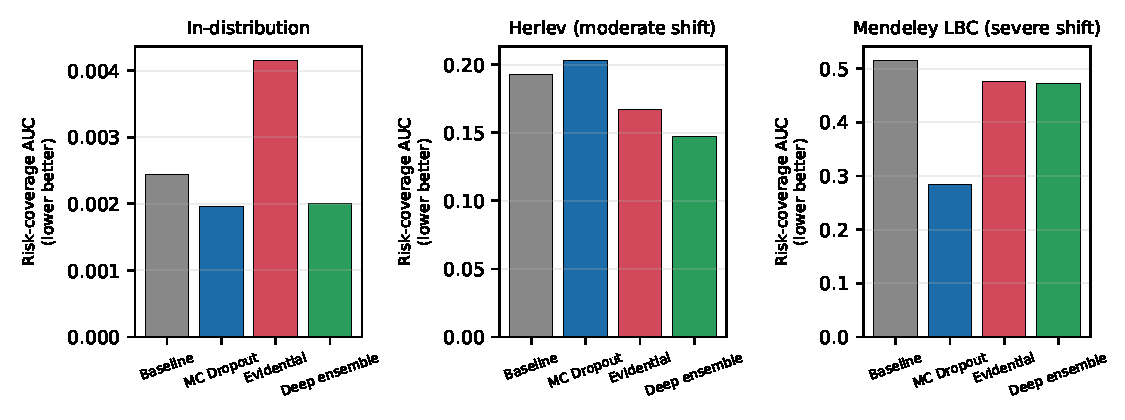
\includegraphics[width=\textwidth]{figs/p2_fig1_risk_coverage.pdf}
\caption{Risk-coverage AUC (lower is better) per method, at three
conditions with independent y-axes (note the $\sim$100$\times$ scale
difference between in-distribution and Mendeley LBC). The best method in
this run changes from deep ensemble (Herlev) to MC Dropout (Mendeley
LBC), though a retraining check found the Mendeley LBC advantage does not
reproduce (see text).}
\label{fig:risk-coverage}
\end{figure}

\textbf{No method reaches a reliable abstention operating point under
severe shift.} Even MC Dropout's best result -- 0.583 selective accuracy
at 90\% coverage on a binary task -- is barely better than chance after
abstaining on the least-confident decile. We report this plainly rather
than treating ``best of four'' as equivalent to ``good enough'': for
deployment purposes, none of these four methods alone would currently
justify an ``abstain and refer'' policy on a shift this severe.

\section{Discussion}

The central methodological finding is that uncertainty-method ranking is
itself a function of shift severity, not a fixed property of the method.
A reader who evaluated these four methods only in distribution, or only
under the milder of the two shifts tested, would conclude the deep
ensemble is the best choice and MC Dropout is mediocre -- the opposite of
what the severe-shift evaluation shows in our original run. This has a
direct practical consequence: a system designer who validates an
uncertainty method under one shift condition and deploys it expecting the
same ranking to hold under a more severe, unseen shift is making an
assumption this data does not support. It also sharpens our companion
architectural finding: no architectural property predicts shift
robustness, and no uncertainty-quantification property predicts
shift-detection quality either, at least not one held fixed across shift
severities.

The significance test (Section~4, ``A significance test, and an
unexpected non-replication'') adds a second, sharper layer to this same
warning. It was not enough for MC Dropout's severe-shift advantage to fail
a bootstrap significance test against the ensemble -- retraining the exact
same method with the exact same seed produced a qualitatively different
result (0.285 becoming 0.503), large enough to flip which method looks
better at all. If a single fixed backbone choice cannot be assumed safe
across shift conditions, and a single fixed uncertainty-method choice
cannot be assumed safe across shift conditions, this result adds a third,
more uncomfortable layer: a single uncertainty-method \emph{evaluation run}
cannot be assumed to represent that method's behavior on a severe shift
either, even holding the seed fixed. Together, these argue that a
trustworthy deployment cannot rely on a single fixed choice validated once
at any of these three levels (backbone, uncertainty method, or a single
training run of that method) and assumed stable -- and that papers
reporting a method comparison from one trained model per method, this one
included, should be read with that specific caveat in mind unless the
comparison has itself been replicated.

\section{Threats to Validity}

\textbf{Internal validity.} This threat is no longer hypothetical for this
paper: we tested it directly by retraining MC Dropout three more times
(seed 13 again, then genuinely different seeds 17 and 29), all under the
identical dropout rate, epoch budget, and manifest used for Table~1. The
four Mendeley LBC risk-coverage AUC values -- 0.285 (Table~1), 0.503, 0.358,
0.359 -- span 0.218, with the two seed-17/29 runs landing in between the
two nominally-seed-13 runs rather than clustering near either. This large
enough swing erases the reported severe-shift advantage entirely and
makes at least one retrained run statistically indistinguishable from the
deep ensemble (paired bootstrap 95\% CI for the difference $[-0.066,
0.010]$, one-sided $p=0.929$; Section~4). The deep ensemble's 5 members
use one fixed set of seeds, reused unchanged for this significance test;
seed-to-seed ensemble variance was not separately measured, so its
risk-coverage AUC at each condition (Table~1) is a point estimate from one
specific ensemble composition, not an average over repeated ensemble
constructions. Table~1's headline Mendeley LBC ranking (MC Dropout 0.285,
evidential 0.476, ensemble 0.473) should accordingly be read as the
result observed for one specific trained instance of each method, not as
a stable per-method property -- four independent MC Dropout training runs
show this is not a theoretical caveat but an empirically demonstrated
failure mode for at least one of the four methods on this exact
condition.

\textbf{External validity.} Single backbone (EfficientViT-M0) and two
shift conditions (Herlev, Mendeley LBC); the paper's central claim --
that uncertainty-method ranking is shift-magnitude-dependent -- is
demonstrated on this specific backbone and these two shifts, not proven
as a general property of uncertainty quantification. Whether the same
rank inversion (ensemble best under moderate shift, MC Dropout best under
severe shift) would recur with a different backbone, a third shift
condition, or a continuous rather than two-point severity scale is
untested and is the most direct follow-up this result motivates.

\textbf{Construct validity.} Risk-coverage AUC and selective accuracy at
fixed coverage are standard selective-prediction metrics with clear
operational meaning (expected error as a function of how much data the
system is willing to abstain on), reducing the risk that the rank
inversion is an artifact of an unusual metric choice. Evidential deep
learning's calibration numbers are reported without the post-hoc
correction its raw outputs would need for a fully fair comparison to the
other three methods' already-calibrated numbers (Section~4, first
paragraph) -- this is a known asymmetry in how the four methods are
scored, stated explicitly rather than smoothed over.

\section{Limitations}

Single backbone (EfficientViT-M0); whether this specific inversion
(ensemble best under moderate shift, MC Dropout best under severe shift)
holds for other architectures is untested. Two shift conditions (Herlev,
Mendeley LBC); ``moderate'' and ``severe'' are descriptive labels based on
the accuracy drop observed, not independently validated shift-magnitude
measurements. Evidential deep learning's calibration numbers are reported
without the post-hoc correction its raw outputs would need for a fully
fair comparison to the other three methods' already-calibrated numbers.
Deep ensemble results depend on the specific 5 seeds used; seed-to-seed
ensemble variance was not separately measured. Most importantly, a direct
retraining check found MC Dropout's reported severe-shift advantage
(Table~1) does not reproduce under an identical seed and recipe (0.503
versus 0.285 risk-coverage AUC on retraining), so the paper's specific
severe-shift ranking should not be treated as a stable per-method result
-- only the higher-level conclusion, that uncertainty-method ranking is
shift-dependent and not safely assumed fixed, is expected to generalize
beyond the single trained model each method's row in Table~1 represents.

\section{Conclusion}

Comparing four uncertainty-quantification methods' own cheapest native
confidence signals on a backbone with a documented real domain-shift
failure shows that method ranking inverts between moderate and severe
shift in our original run: deep ensembles win under moderate shift, MC
Dropout wins under severe shift, and neither method's advantage transfers
to the other condition. A follow-up significance test then complicated
this result rather than confirming it: retraining MC Dropout under an
identical seed and recipe did not reproduce its reported severe-shift
advantage at all, and the retrained run is statistically indistinguishable
from the deep ensemble. No method reaches a reliable abstention operating
point under the severe shift condition that matters most, in either run.
The practical conclusion now has two layers rather than one: a single
fixed uncertainty-quantification method, chosen and validated once, cannot
be assumed to remain the right choice as shift severity varies; and, more
sharply, a single trained instance of that method, evaluated once under
one severe-shift condition, cannot be assumed to represent that method's
behavior even under an identical seed and recipe. Both need to be tested,
not assumed, for any deployed system relying on model confidence to
decide when to abstain -- and any single-run method comparison, including
this paper's own headline numbers, should be read with that caveat
attached.

\begin{thebibliography}{99}

\bibitem{guo2017calibration}
Guo, C., Pleiss, G., Sun, Y., Weinberger, K.Q.: On calibration of modern
neural networks. In: ICML (2017)

\bibitem{gal2016dropout}
Gal, Y., Ghahramani, Z.: Dropout as a Bayesian approximation:
Representing model uncertainty in deep learning. In: ICML (2016)

\bibitem{lakshminarayanan2017ensembles}
Lakshminarayanan, B., Pritzel, A., Blundell, C.: Simple and scalable
predictive uncertainty estimation using deep ensembles. In: NeurIPS (2017)

\bibitem{sensoy2018evidential}
Sensoy, M., Kaplan, L., Kandemir, M.: Evidential deep learning to
quantify classification uncertainty. In: NeurIPS (2018)

\end{thebibliography}
\end{document}
